% What I want to cover in these sections is the following:
% - General introduction to the problem: approximation of fading models with GANs, which are highly complex.
% - Motivation: approximating the MFTR is the first step before repeating the same procedure with empirical data. 
% The end goal is to learn an empirical distribution estimating the parameters of each data point, and then generate new sample points with different paramters.
% This requires our gan to be able to interpolate and extrapolate.
% - Related work: brief description of other papers that have attempted to approximate 1D distributions using GANs.
The estimation of an underlying probability distribution from data is a fundamental problem in many fields, including wireless communications. Since a population can be fully characterized by its probability distribution, being able to estimate this distribution from data is crucial for understanding and modeling complex phenomena, generate new samples, and make predictions under given conditions, say for instance environmental factors related to the propagation of radio signals across a medium.

On way to do so is to use Generative Adversarial Networks (GANs), a family of generative models that generate new samples from a target distribution by implicitly learning their underlying distribution \cite{goodfellow2014generativeadversarialnetworks}. They consist of two neural networks, a generator and a discriminator, that are trained in an adversarial manner. The generator takes random noise as input and produces synthetic samples, while the discriminator tries to distinguish between real and fake samples. Through this process, the generator learns to produce samples that are indistinguishable from real data. GANs have been successfully applied in various domains, including image generation \cite{karras2019stylebasedgeneratorarchitecturegenerative}, time series simulation \cite{fu2019time} and audio synthesis \cite{donahue2019adversarialaudiosynthesis}.

In this work, we focus our attention in a variant of GANs called conditional GANs (cGANs), which allow for the generation of samples conditioned on specific input variables, enabling more control over the generated data \cite{mirza2014conditional}. Although the original cGANs paper uses categorical labels as the condition input, there have been several works that have successfully used continuous variables as conditions, such as \cite{fu2019time} and \cite{zaheer2017gan}. Our goal is to use them to approximate the distribution of a complex fading model, the Multi-Cluster Fluctuating Two-Ray (MFTR) fading model \cite{sánchez2023multiclusterfluctuatingtworayfading}. 

The MFTR model is a generalization of the Fluctuating Two-Ray (FTR) fading model and the $\kappa-\mu$ fading model, all of which attempt to model the amount of power received at a given location when a radio signal travels and interacts with the environment in several ways. It depends on 5 parameters, $\Delta, m, \mu, K, \bar{\gamma}$ (see Fig. \ref{fig:mftr_mu_cases}) that allow extensive control of the shape of the distribution, including a transition from an unimodal to a bimodal distribution, which makes it a good candidate for testing the ability of cGANs to learn complex distributions.

\begin{figure}[h]
    \centering
    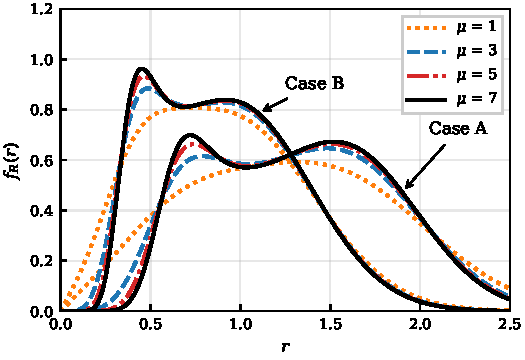
\includegraphics[width=0.9\columnwidth]{../images/mftr_mu_cases.pdf}
    \caption{PDF of the MFTR signal envelope by varying $\mu$ in two different scenarios: Case A: $\Delta = 0.9$, $m = 8$, $K = 8$, $\bar{\gamma} = 2$ and Case B: $\Delta = 0.9$, $m = 4$, $K = 15$, $\bar{\gamma} = 1$. Reproduced from \cite{sánchez2023multiclusterfluctuatingtworayfading}.}
    \label{fig:mftr_mu_cases}
\end{figure}

This work is a first step towards the ultimate goal of learning an empirical distribution from real data taken from experiments on wireless channels, which would allow us to generate new samples with different parameters. This requires our GAN to be able to interpolate and extrapolate, which we explore in the following sections.